\section{Dynamic Model}
\label{sec:dynamic_model}

Earth rotation synthesis inherently assumes that the source being imaged is static over the course of an observation~\cite{taylor1999synthesis}. 
%Generally, this makes it possible to collect multiple measurements that inform us about the same underlying image. 
If this assumption holds, it is possible to collect more than $\ntele (\ntele-1)/2$ measurements that inform us about the underlying source through earth rotation synthesis
However, in the case of an evolving source, as is predicted to be the case for SgrA*, this assumption is violated -- measurements taken at different times throughout the observation correspond to different underlying source images. 

At each time $t=1,...,\ntime$ we measure a vector of data products $\meas_t$, that are observed
%generated 
from an evolving source image, $\im_t$. Our goal is to reconstruct the $\ntime$ instantaneous images $ {\bf X} = \{\im_1, ..., \im_\ntime \}$ using the set of sparse observations $ {\bf Y} = \{\meas_1, ..., \meas_\ntime \}$. We define a dynamic imaging %generative (?)
model for this observed data as potentials ($\varphi$) of an undirected tree graph (see Figure~\ref{fig:model}):
\begin{align}
\varphi_{\meas_t | \im_t} &=  \mathcal{N}_{\meas_t} ( f_t ( \im_{t} ) , \bR_t ), \\
\varphi_{\im_t} &=  \mathcal{N}_{\im_1} ( \bmu_t, \bLambda_t ), \\
\varphi_{\im_t|\im_{t-1}} &=  \mathcal{N}_{\im_t} ( \evolve \im_{t-1}, \bQ ), 
\label{eq:evolution_potential}
\end{align}
for $\bLambda_t = \mathrm{diag}[\bmu_t]^T \bLambda'\mathrm{diag}[\bmu_t]$. 


Similar to the static imaging model, each set of observed data $\meas_t$ taken at time $t$ is related to the underlying instantaneous source image, $\im_t$, through the functional relationship, $f_t(\im_t)$, and $\im_t$ is encouraged to be a sample from a multivariate Gaussian distribution. However, new to this dynamic imaging model is the addition of (\ref{eq:evolution_potential}) that describes how images evolve over time. 
%The final set of terms involving the evolution matrix, $A$, define how the underlying image evolves over time. 
If we assume that there is no evolution between neighboring images in time ($\evolve=\mathds{1}, \bQ = \bm{0}$), this dynamic model reduces to that of static imaging. 
Using the Hammersley-Clifford Theorem~\cite{hammersley1971markov}, the joint distribution of this dynamic model can be written as a product of its potential functions: 
\begin{align}
p({\bf X}, {\bf Y} ; \evolve )  \propto \prod_{t=1}^{\ntime} \varphi_{\meas_t |\im_t} \prod_{t=1}^{N} \varphi_{\im_t}   \prod_{t=2}^{\ntime} \varphi_{\im_t|\im_{t-1}} .
\label{eq:likelihood}
\end{align}

% \begin{align}
%  & p({\bf X}, {\bf Y} | \evolve ) =  p(\im_1, ..., \im_N, \meas_1, ..., \meas_\ntime | \evolve )    \\
% \notag & \propto \prod_{t=1}^{\ntime} \mathcal{N}_{\im_1} ( \bmu_t, \bLambda_t ) \prod_{t=1}^{N}  \mathcal{N}_{\meas_t} ( \FTmtx_t \im_{t} , \bR_t ) \prod_{t=2}^{\ntime}  \mathcal{N}_{\im_t} ( \evolve \im_{t-1}, \bQ )
% \end{align}

% \begin{align}
%  & p({\bf X}, {\bf Y} | \evolve ) =  p(\im_1, ..., \im_N, \meas_1, ..., \meas_\ntime | \evolve )    \\
% \notag & = \mathcal{N}_{\im_1} ( \bmu, \bLambda ) \prod_{t=1}^{N}  \mathcal{N}_{\meas_t} ( \FTmtx_t \im_{t} , \bR_t ) \prod_{t=2}^{\ntime}  \mathcal{N}_{\im_t} ( \evolve \im_{t-1}, \bQ )
% \end{align}


% \begin{align}
%  p({\bf X}, {\bf Y} | \theta ) &= \mathcal{\ntime}_{\im_1} ( \bmu, \bLambda ) \prod_{t=1}^{\ntime}  \mathcal{N}_{\meas_t} ( \FTmtx_t \im_{t} , \bR_t )  \\
%  & s.t. \hspace{0.1in} \im_1 = \im_2 = ... = \im_\ntime
% \end{align}

% By vertically stacking each matrix $\FTmtx_t$ into a matrix $\FTmtx$ and placing $\bR_t$ along the diagonal of matrix $\bR$, we can calculate the most likely estimate of each $\im_t$ using Weiner filtering (refer to Equation BLAH).

% \begin{align}
% \hat{x}_t &=  \bmu  + \bLambda \FTmtx^T ( \bR + {\bf F} \bLambda \FTmtx^T )^{-1} (  y -  \FTmtx \bmu ) \hspace{.12in} \forall t \in 1,...,N
% \end{align}




%\subsection{Observation Model} 



%\paragraph{Linear Observations} As mentioned in Section BLAH, the visibilities measured by an interferometer are related to the underlying image via a Fourier transform. Thus, for simplicity, we first assume that we are able to measure complex visibilities with Gaussian noise.  relationship is linear and each measurement can be expressed as $y_t + \mbox{noise} = f_t(x_t) = F_t x_t$ for DTFT matrix $F_t$. 


%\paragraph{Non-linear Observations} However, as mentioned in Section BLAH the complex visibilities often have large atmospheric noise that make them   
%we often do not have access to complex vi
%For simplicity, we first present derivations assuming a linear observation model. In Section BLAH we specify how to handle non-linear relationships, such as must be used in the case of constraining phase-closure.


\begin{figure}
	\centering
	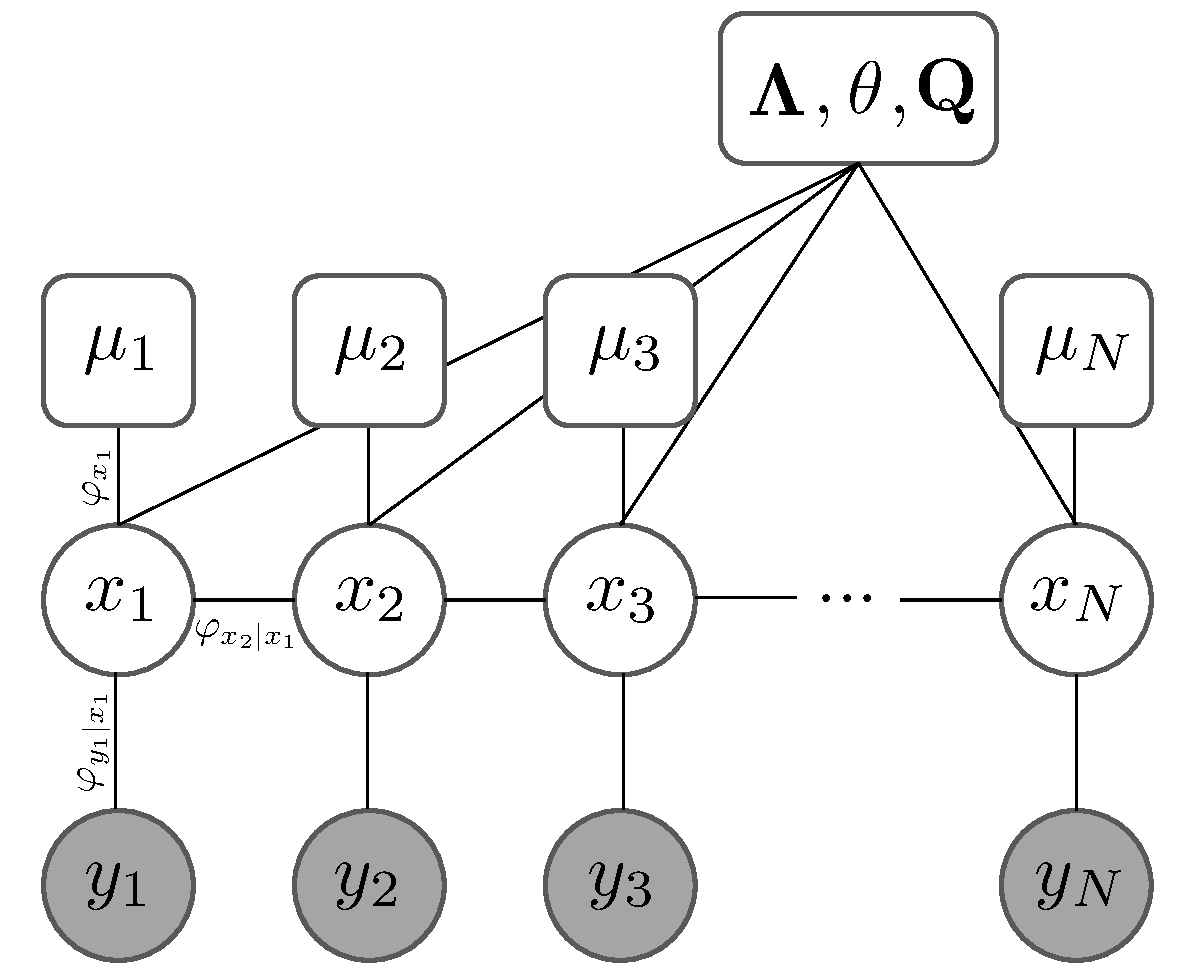
\includegraphics[width=0.8\linewidth]{figures/graphicalmodel_2.pdf}
\caption{{\bf Graphical Representation of our Dynamic Imaging Model}: At each time $t$ we observe a vector of data products $\meas_t$ corresponding to the instantaneous source image $\im_t$. 
	%To solve for the set of latent images $\bm{X} = \{ \im_t\}_{t=1}^N$ 
	We assume each image $\im_t$ is related to its adjacent neighbors in time, $\im_{t-1}$ and $\im_{t+1}$, and is also related to a multivariate Gaussian distribution specified by mean $\bmu_t$ and covariance $\bLambda$. The persistent global evolution of the source images over time is specified by $\evolve$, which is further parameterized by $\theta$. Additional intensity perturbations in time are constrained by the covariance matrix $\bQ$. In this diagram, squares indicate parameters, circles are variables, and shaded circles indicate the variable is observed. }
\label{fig:model}
\vspace{-.2in}
\end{figure}









\vspace{-.2in}
\subsection{Evolution Model}
\label{sec:evolution}

Each image $\im_t$ is related to the previous image $\im_{t-1}$ through a linear relationship: $\im_t \approx \evolve \im_{t-1}$.  Matrix $\evolve$ (size $\npix^2 \times \npix^2$) %and $B$ (size $M^2 \times 1$)
defines the evolution of the source's emission region between time steps.
 For instance, $\evolve=\mathds{1}$ indicates that, on average, the source image does not change, whereas $\evolve=2 \mathds{1}$ indicates that the image's brightness doubles at each time step. Since the evolution matrix $\evolve$ is not time dependent, the underlying source image evolves similarly over the entire observation. However, at each time the image can deviate slightly from this persistent evolution. 
 %The amount of allowed deviation 
 The amount of allowed intensity deviation is expressed in the time-invariant covariance matrix $\bQ$.  
%We refer to this property as persistent flow.

We assume that the evolution of the emission region over time is primarily described by small perturbations on top of a persistent 2D projected flow of material that preserves total flux.
We treat each source image like a 2D array of light pulses originating at locations $( \bm{\xpos}, \bm{\ypos})$. These pulses can shift around, causing motion in the image. %resemble
As described by the Shift Theorem, the shift of a pulse by $\Delta$ will change the phase of its Fourier Transform by $2 \pi f \Delta$ for each frequency $f$. % can be related to its phase in the frequency domain.
%As described by the Shift Theorem, the position of a pulse can be related to its phase in the frequency domain
Thus, under small motions, we can write $\evolve$ in terms of the image's full $M^2 \times M^2$ DFT matrix $\bm{W}$ (see Section~\ref{sec:gauss_prior}), and a column-vector of $M$ pixel shifts: $\bm{s} = (\bm{s}_{ \bm{\xpos}}, \bm{s}_{\bm{\ypos}})$:
%As the position of a pulse can be related to its phase in the frequency domain, under small motions we write $\evolve$ in terms of the image's full DTFT matrix $\bm{W}$, and a column-vector of pixel shifts: $\bm{s} = (\bm{s}_{ \bm{\xpos}}, \bm{s}_{\bm{\ypos}})$. \katie{check if there should be a negative in the exponent}
\begin{align}
\evolve = \Re \left[ \bm{W}^{*T} \hspace{0.01in}  \left(  \exp \left[ -i 2 \pi ( \bm{u} \bm{s}_{\xpos}^T + \bm{v} \bm{s}_{\ypos}^T ) \right]  \odot  \bm{W}  \right) \right] . 
\end{align}
Applying $\evolve$ to a vectorized image $\im_t$ of light pulses results in a new image, $\im_{t+1}$, where the pulses have been shifted according to $\bm{s}$ and re-interpolated on the 2D DFT grid. Note that in the case $\bm{s} = \bm{0}$ then $\evolve = \bm{W}^{*T} \bm{W} = \mathds{1}$.

%Note that in the case $\bm{s} = \bm{0}$ then $\evolve = \bm{W}^{*T} \bm{W} = \mathds{1}$, and that the same 2D DFT grid locations  image $\im_{t+1}$

%Note that in the case $\bm{s} = \bm{0}$ then $\evolve = \bm{W}^{*T} \bm{W} = \mathds{1}$, and that this $\evolve$ matrix results in new light pulses being defined at the same 2D DFT grid locations after the old pulses have been shifted. 

%\vspace{0.1in}
%\subsubsection{Low-Dimensional Motion Basis}

The above parameterization of evolution matrix $\evolve$ in terms of $\bm{s}$ allows for independent, arbitrary shifts of each pulse of light, resulting in $2 \npix^2$ shift parameters. However, as neighboring material generally moves together, the pixel shifts should have a much lower intrinsic dimensionality. 
%BLAH BLAH BLAH. 
%Additionally, during inference solving for the $2 M^2$ parameters of $\bm{s}$. 
%However, solving this problem is very ill-posed because the number of unknowns, $s$, (number of pixels) far exceeds the number of measurements, $\vis$, for a single time step. 
To address this, and simultaneously reduce the number of free parameters, we instead describe motion $\evolve$ using a low-dimensional subspace, parameterized by $\theta$. The length of $\theta$, $D$, is much smaller than the number of unconstrained shift parameters, $2 \npix^2$. %: $\evolve(\theta)$. 
We define a motion basis $\mathcal{M} = \Spvek{\mathcal{M}_{\xpos}, \mathcal{M}_\ypos}^T$ of size $2\npix^2 \times D+1$, and restrict the motion at every time step to be a linear function of this motion:
\begin{align}
\Spvek{\bm{\xpos}_{t+1}; \bm{\ypos}_{t+1}} = \Spvek{\bm{\xpos}_t; \bm{\ypos}_t} + \Spvek{\bm{s}_{\xpos_t}; \bm{s}_{\ypos_t}} =  \Spvek{\mathcal{M}_{\xpos_t}; \mathcal{M}_{\ypos_t}} \Spvek{1; \theta} .
\end{align}
%where $\bm{\xpos}_t$ and $\bm{\ypos}_t$ indicate the two-dimensional position of each pulse at time $t$. Note that the $\evolve$ matrix defined above results in new light pulses being defined at the same 2D DFT grid locations after the old pulses have been warped. 

This parameterization allows us to describe a wide variety of motion (or warp) fields. 
Generic ``smooth" warp fields can be described by using a truncated Discrete Cosine Transform (DCT) basis as $\mathcal{M}$.
However, more compressed motion bases can also be used~\cite{lowdim14, erikmiller}. 
In this work, results are shown using an affine transformation parametrized with a four-dimensional $\theta$ that captures rotation, shear, and scaling. As an affine transformation, $\theta$, acting on a pulse at location $(\xpos_t, \ypos_t)$ results in moving the pulse to location
%fit into this framework. 
    \begin{align}
    \Spvek{{\xpos}_{t+1}; {\ypos}_{t+1}} = \Spvek{\theta_1 \hspace{.1in}\theta_2 ; 
    	\theta_3 \hspace{.1in}\theta_4  } \Spvek{{\xpos}_{t}; {\ypos}_{t}} = \Spvek{ \xpos_t \hspace{.1in} \ypos_t \hspace{.1in}0 \hspace{.1in} 0 ; 
    	0 \hspace{.1in}0 \hspace{.1in} \xpos_t \hspace{.1in} \ypos_t } \Spvek{\theta_1; \theta_2; \theta_3; \theta_4},
    \end{align}
 in this work we define, 
   \begin{align}
  \Spvek{\mathcal{M}_{\xpos_t}; \mathcal{M}_{\ypos_t}}  =  \Spvek{\bm{0} \hspace{.1in} \bm{\xpos}_t \hspace{.1in} \bm{\ypos}_t \hspace{.1in} \bm{0} \hspace{.1in} \bm{0} ; \bm{0} \hspace{.1in}
   	\bm{0} \hspace{.1in} \bm{0} \hspace{.1in} \bm{\xpos}_t \hspace{.1in} \bm{\ypos}_t } .
   \end{align}
For example, using this motion basis with $\theta_1 = \cos \phi$, $\theta_2 = \sin \phi$, $\theta_3 = -\sin \phi$, and $\theta_4 = \cos \phi$ would specify that every time step the image is rotated by $\phi$ radians. 


%This parameterization allows us to describe a wide variety of motion (or warp) fields. For instance, affine transformation can be parametrized with a six-dimensional $\theta$ that captures rotation, shear, translation, and scaling.
%fit into this framework. 
%More general warp fields can also be described by using a truncated Discrete Cosine Transform (DCT) basis as $\mathcal{M}$. 


% \paragraph{Affine Motion Basis}

% An affine transformation is able to capture rotation, shear, translation, and scaling. It can be written in terms of a six dimensional vector $\theta$, where $\theta = \Spvek{1, 0, 0, 0, 1, 0}^T$ would be equivalent to no transformation. 

%   \begin{align}
%   \Spvek{\xpos_{t+1}; \ypos_{t+1}} = \Spvek{\xpos_t \hspace{.1in}\ypos_t \hspace{.1in} 1 \hspace{.1in}0 \hspace{.1in} 0 \hspace{.1in} 0; 
%   	0 \hspace{.1in}0 \hspace{.1in} 0 \hspace{.1in} \xpos_t \hspace{.1in} \ypos_t \hspace{.1in} 1} \theta
%   \end{align}

% \paragraph{Smooth Motion Basis} $\bm{D'} = (\FTmtx[ \sqrt{\bm{u}^2 + \bm{v}^2} <\tau,:])^T$


%    \begin{align}
%   \Spvek{\bm{\xpos}_{t+1}; \bm{\ypos}_{t+1}} = \Spvek{ \Re (\bm{D'}) \Im( \bm{D'} ); \Re (\bm{D'}) \Im( \bm{D'} ) } \theta
%   \end{align}



\section{Dynamic Imaging Inference \& Learning}
\label{sec:dynamic_inference}


%The dynamical observation model presented in Section BLAH can be thought of as an undirected graphical model. Refer to Figure BLAH. 


We solve for the best set of $\ntime$ images $ \bm{X} $ constrained by the $\ntime$ vectors of sparse observations $\bm{Y}$. In general, we assume that $f_t(.)$, $\bR_t$, $\bmu_t$, $\bLambda_t$, $\bQ$ are known/specified model parameters. However, $\evolve$, which defines how the source evolves, is not necessarily known ahead of time. If there is reason to believe that only small perturbations exist in the source image over time, then a reasonable assumption is to set $\evolve = \mathds{1}$. However, in the case of large persistent motion this may fail to give informative results. 

We begin in Section~\ref{sec:dynamic_inference_known} by discussing how to solve for $\bm{X}$ when $\evolve$ is known. In this case, the model contains no unspecified parameters and the goal is to simply solve for the latent images. 
In Section~\ref{sec:dynamic_inference_unknown}, we forgo this assumption and no longer assume that $\evolve$ is known. In this case, we jointly solve for $\evolve$ and $\bm{X}$ by first learning $\evolve$'s parameters $\theta$ using an Expectation-Maximization (EM) algorithm before solving for the latent images, $\bm{X}$. We refer to our proposed method as StarWarps. 
%{\bf MDJ: We might want to change the language from "the model contains no unknown parameters" to "the model contains no unspecified parameters". Similar to Kazu's point, we should emphasize what parameters the user must specify in an ad hoc fashion.}













\subsection{Known Evolution}
\label{sec:dynamic_inference_known}

Given all of the model parameters and observed data, our goal is to estimate the optimal set of latent images, $\bm{X}$. 
In static imaging we set up an optimization problem that allowed us to easily solve for the most likely latent image, $\im$, given the observed data, $\meas$. 
In the proposed dynamic model, a similar closed-form solution exists in the case of a linear $f(\im)$ and diagonal $\bR_t$ and $\bQ$ matrices~\cite{fessler}. However, this requires us to invert a large $\npix^4 \times \ntime^2$ non-block-diagonal matrix.   
Thus, instead of the MAP estimate, we compute the most likely instantaneous image at each time, $t$, given all of the observed data $\bm{Y}$.
In particular, we estimate the marginal distribution of each $\im_t$, $p(\im_t | \bm{Y})$, by integrating out the other latent images in time, and set $\hat{\im}_t$ equal to the mean of each distribution. 

%Given all of the model parameters and observed data, our goal is to estimate the optimal set of latent images, $\bm{X}$. 
%In static imaging we set up an optimization problem that allowed us to easily solve for the most likely latent image, $\im$, given the observed data, $\meas$. 
%However, in the proposed dynamic model, solving for a MAP estimate -- the set of all images that maximizes Equation~\ref{eq:likelihood} -- is much more difficult, as a closed-form solution does not exist. 
%Instead of the MAP estimate, we compute the most likely instantaneous image at each time, $t$, given all of the observed data $\bm{Y}$.
%In particular, we estimate the marginal distribution of each $\im_t$, $p(\im_t | \bm{Y})$, by integrating out the other latent images in time, and set $\hat{\im}_t$ equal to the mean (and mode) of each distribution. 


%Instead, we take the approach of solving for the marginal distribution of each $\im_t$ and setting $\hat{\im}_t$ equal to the mean (and mode) of each distribution. Although this does not necessarily produce the MAP estimate under our model, it provides the most likely instantaneous image at each time, $t$, given all of the observed data $\bm{Y}$.


Since we have defined our dynamic model in terms of Gaussian distributions, we can efficiently solve for $p(\im_t | \meas_1,...,\meas_\ntime)$ by marginalizing out the latent images $ \{ \im_1,...,\im_{t-1},\im_{t+1},...,\im_{\ntime} \}$ using the Elimination Algorithm~\cite{graphicalmodels}. Specifically, we derive a function proportional to the marginal distributions. This function is evaluated using a two-pass algorithm, which consists of a forward pass and a backward pass. Each pass, outlined in Algorithms~\ref{alg:forward} and~\ref{alg:backward}, propagates information using recursive updates that compute distributions proportional to 
%$p(\im_t | \meas_1,...,\meas_{t-1})$ and $p(\im_t | \meas_{t},...,\meas_{\ntime})$ 
$p(\im_t, \meas_1,...,\meas_{t-1})$ and $p( \meas_{t},...,\meas_{\ntime} | \im_t )$ 
for each $\im_t$ in the forward and backward pass, respectively. By combining these terms we obtain
\begin{align}
\label{eq:marg1}
p(\im_t|\bm{Y}) & = \mathcal{N}_{x_t}(\hat{\im}_t, \bm{C}_t ) \\
\notag & \propto \mathcal{N}_{x_t}({\bf z}^{\alpha}_{t|t-1}, {\bf P}^{\alpha}_{t|t-1})  \mathcal{N}_{x_{t}}( {\bf z}^{\beta}_{t|t} , {\bf P}^{\beta}_{t|t} ),
\end{align}
which, as shown in the supplemental material, has mean $\hat{\im}_t$ and covariance $\bf{C}_t$:
{\footnotesize
	\begin{align}
	\notag    \hat{\im}_t & = {\bf P}^{\beta}_{t|t} ( {\bf P}^{\alpha}_{t|t-1} + {\bf P}^{\beta}_{t|t})^{-1} {\bf z}^{\alpha}_{t|t-1}  +   {\bf P}^{\alpha}_{t|t-1}( {\bf P}^{\alpha}_{t|t-1} + {\bf P}^{\beta}_{t|t})^{-1} {\bf z}^{\beta}_{t|t} \\
	\bf{C}_t & =  {\bf P}^{\alpha}_{t|t-1}( {\bf P}^{\alpha}_{t|t-1} + {\bf P}^{\beta}_{t|t})^{-1} {\bf P}^{\beta}_{t|t} , 
	\label{eq:marg2}
	\end{align}
}where ${\bf z}_{t|\tau}^{\alpha}$, ${\bf P}_{t|\tau}^{\alpha}$ are the estimates of the mean and covariance of $\im_t$ using observations at time steps $1$ through $\tau$. Similarly, ${\bf z}_{t|\tau}^{\beta}$, ${\bf P}_{t|\tau}^{\beta}$ are the estimates of the mean and covariance of $\im_t$ using observations $\tau$ through $\ntimes$.



For generality, we have listed the forward and backward algorithms in terms of non-linear measurement functions, $f_t(\im_t)$ with derivative $\dot{\FTmtx}$. In this case, similar to our static model inference in Section~\ref{sec:static_inf}, we linearize the solution around $\tilde{\im}_t$ to get an approximate estimate. To improve the solution of the forward and backward terms, each step in the forward pass can be iteratively re-solved, updating $\tilde{\im}_t$ at each iteration. The values of $\tilde{\im}_t$ are then fixed for the backwards pass. Recall %from Section BLAH 
that when $f_t(\im)$ is linear in $\im$ then $f_t(\im) = \FTmtx_t \im  = \dot{\FTmtx}_t \im$, and the $\hat{\im}$ will converge to the optimal solution in a single update.

The above inference algorithm is similar to %Kalman filtering and smoothing for Linear Dynamical Systems. 
the forward-backward algorithm used for Gaussian Hidden Markov Models~\cite{graphicalmodels}. 
In fact, removing the $\varphi_{\im_t}$ term for $t>1$ in Equation~\ref{eq:likelihood} yields the familiar form of a Gaussian Hidden Markov Model. In this case, inference reduces to the traditional Kalman filtering and smoothing (extended Kalman filtering in the case of non-linear $f_t(\im)$)~\cite{anderson1979optimal}. Although this simpler formulation can sometimes produce acceptable results, in our typical scenario of especially sparse or noisy data keeping the additional potential terms helps to further constrain the problem, and results in better reconstructions. 
%For derivations in the case of a Hidden Markov Model, see the supplemental material. 

\RestyleAlgo{boxruled}
\begin{algorithm}[t]
	\caption{Forward Updates {\footnotesize $t = 1 \rightarrow 2 \rightarrow ... \rightarrow \ntime$ } \label{alg:forward} }
	
	{\bf Predict:}
	
	{ \footnotesize
		\begin{align}
		\notag {\bf z}^{\alpha}_{t|t-1} &= \evolve {\bf z}^{\alpha}_{t-1|t-1} \\
		\notag {\bf P}^{\alpha}_{t|t-1} &= \bQ  + \evolve {\bf P}^{\alpha}_{t-1|t-1} \evolve^T
		\end{align}
		\begin{align}
		\notag {\bf z}^{\alpha*}_{t|t-1} &= \bLambda_t ( \bLambda_t + {\bf P}^{\alpha}_{t|t-1} )^{-1} {\bf z}^{\alpha}_{t|t-1} + {\bf P}^{\alpha}_{t|t-1} ( \bLambda_t + {\bf P}^{\alpha}_{t|t-1} )^{-1} \bmu_t \\
		\notag {\bf P}^{\alpha*}_{t|t-1} & = \bLambda_t ( \bLambda_t + {\bf P}^{\alpha}_{t|t-1} )^{-1} {\bf P}^{\alpha}_{t|t-1} 
		\end{align}
	}
	
	{\bf Update:}
	
	{\footnotesize
		\begin{align}
		\notag \meas_\Delta &= (  \meas_t + \dot{\FTmtx} \tilde{\im}_t - f(\tilde{\im}_t) -  \dot{\FTmtx} {\bf z}^{\alpha*}_{t|t-1} ) \\
		\notag {\bf z}^{\alpha}_{t|t} &  =  {\bf z}^{\alpha*}_{t|t-1}  + {\bf P}^{\alpha*}_{t|t-1} \dot{\FTmtx}_t^T ( \bR_t +  \dot{\FTmtx}_t {\bf P}^{\alpha*}_{t|t-1} \dot{\FTmtx}_t^T )^{-1} \meas_\Delta  \\
		\notag {\bf P}^{\alpha}_{t|t} & = {\bf P}^{\alpha*}_{t|t-1} - {\bf P}^{\alpha*}_{t|t-1}\dot{\FTmtx}_t^T ( \bR_t + \dot{\FTmtx}_t {\bf P}^{\alpha*}_{t|t-1} \dot{\FTmtx}_t^T )^{-1} \dot{\FTmtx}_t {\bf P}^{\alpha*}_{t|t-1} 
		\end{align}
	}
	
	
	{\bf Initialization:}
	
	{\footnotesize
		\begin{align}
		\notag {\bf z}^{\alpha*}_{1|0} = \bmu_1 \mbox{   ,   } {\bf P}^{\alpha}_{1,0}   = \bLambda_1
		\end{align}
	}
	
	
\end{algorithm}


\RestyleAlgo{boxruled}
\begin{algorithm}[b]
	\caption{Backward Updates: {\footnotesize $t = \ntime \rightarrow \ntime-1 \rightarrow ... \rightarrow 1 \hspace{-.1in}$ }  \label{alg:backward}}
	
	{\bf Predict:}
	{\footnotesize
		\begin{align}
		\notag {\bf z}^{\beta*}_{t|t+1}  & \hspace{-.02in} = \hspace{-.02in} \bmu_t  + \bLambda_t  \evolve^T ( \bQ + {\bf P}^{\beta}_{t+1|t+1} +  \evolve \bLambda_t  \evolve^T )^{-1} (  {\bf z}^{\beta}_{t+1|t+1} \hspace{-.13in} -   \evolve \bmu_t ) \\
		\notag  {\bf P}^{\beta*}_{t|t+1} &  \hspace{-.02in}= \hspace{-.02in} \bLambda_t - \bLambda_t \evolve^T (  \bQ + {\bf P}^{\beta}_{t+1|t+1} + \evolve \bLambda_t  \evolve^T )^{-1}  \evolve \bLambda_t 
		\end{align}
	}
	
	
	{\bf Update:}
	
	{\footnotesize
		\begin{align}
		\notag \meas_\Delta &= (  \meas_t + \dot{\FTmtx} \tilde{\im_t} - f(\tilde{\im}_t) -  \dot{\FTmtx}_t {\bf z}^{\beta*}_{t|t+1} ) \\
		\notag  {\bf z}^{\beta}_{t|t} &  =  {\bf z}^{\beta*}_{t|t+1}  + {\bf P}^{\beta*}_{t|t+1} \dot{\FTmtx}_t^T ( \bR_t +  \dot{\FTmtx}_t {\bf P}^{\beta*}_{t|t+1} \dot{\FTmtx}_t^T )^{-1} \meas_\Delta \\
		\notag  {\bf P}^{\beta}_{t|t} & = {\bf P}^{\beta*}_{t|t+1} - {\bf P}^{\beta*}_{t|t+1}\dot{\FTmtx}_t^T ( \bR_t + \dot{\FTmtx}_t {\bf P}^{\beta*}_{t|t+1} \dot{\FTmtx}_t^T )^{-1} \dot{\FTmtx}_t {\bf P}^{\beta*}_{t|t+1} 
		\end{align}
	}
	
	
	{\bf Initialization:}
	
	{\footnotesize
		\begin{align}
		\notag  {\bf z}^{\beta*}_{\ntime|\ntime+1} = \bmu_{\ntime} \mbox{   ,   } {\bf P}^{\beta*}_{\ntime|\ntime+1}   = \bLambda_{\ntime}
		\end{align}
	}
	
	
\end{algorithm}


\vspace{-.1in}

\subsection{Unknown Evolution}
\label{sec:dynamic_inference_unknown}

% \subsection{Inference With Known Evolution}

% In general, we do not know how an emission evolves over time. T
% In this model, we assume that $f_t, \bR_t, \bQ, \mu$, and $\bLambda$ are known, but matrix $A$ is unknown.

% \subsection{Inference Without Known Evolution}

If the evolution matrix $\evolve$ is unknown, it is not possible to simply solve for $\bm{X}$ in the way outlined in Section~\ref{sec:dynamic_inference_known}. 
%In theory, although it is possible to compute a gradient of Equation~\ref{eq:likelihood} with respect to each $\bm{X}$ and $\evolve$ and perform gradient ascent, this would be very computationally intensive and prone to local maxima. This becomes even more pronounced when solving for the evolution parameters $\theta$ (see Section~\ref{sec:evolution}) rather than $\evolve$ itself. 
Instead we choose to use an Expectation-Maximization (EM) algorithm to recover $\evolve$ (parameterized by $\theta$), and then subsequently use the procedure presented in Section~\ref{sec:dynamic_inference_known} to recover $\bm{X}$. 
%Instead we choose to jointly solve for latent images $\bm{X}$ and parameters $\evolve$ (parameterized by $\theta$) using the Expectation-Maximization (EM) algorithm. 
%The EM algorithm defines an iterative process that allows us to maximize the likelihood function of a parametric model in the case in which some variables of the model are "latent" or unknown. 

The EM algorithm defines an iterative process that
solves for 
%helps us to find 
the evolution parameters $\theta$ that maximize the complete likelihood in Equation~\ref{eq:likelihood} when all of the underlying images, $\bm{X}$, are unknown (latent). 
Each iteration of EM improves the log-likelihood of the data under the defined objective function and is especially useful when the likelihood is from an exponential family, as is the case in our proposed model. In particular the EM algorithm consists of the following two iterative steps:

\begin{itemize}
	\item Expectation step (E step): Calculate the expected value of the log likelihood function (see Equation~\ref{eq:likelihood}), with respect to the conditional distribution of $\bm{X}$ given $\bm{Y}$ under the current estimate of the $\theta$ parameters, $\theta^{(i)}$: %$Q(\theta|\theta^{(i)} = E_{X|Y, \theta^{(i}} [ \log L (\theta, Y, X) ]$.
	\begin{align}
	Q(\theta|\theta^{(i)}) = E_{ {\bf X}| {\bf Y}, \theta^{(i)}} [ \log p ({\bf X}, {\bf Y} | \theta) ]
	\label{eq:qfunction}
	\end{align}
	\item Maximization step (M step): Find the parameter that maximizes: %$\theta^{(i+1)} = \argmax_{\theta} Q(\theta | \theta^{(i)} )$.
	\begin{align}
	\theta^{(i+1)} = \argmax_{\theta} Q(\theta | \theta^{(i)} ) .
	\label{eq:argmaxem}
	\end{align}
\end{itemize}

We solve for $\theta$ using gradient ascent. As $\evolve$ is a function of $\theta$, we must %solve for the optimal $\theta$ we must first 
compute the derivative of $Q(\theta|\theta^{(i)})$ using the chain rule. We compute this derivative with respect to each element $j$ in $\theta$: 
\begin{align}
\frac{d}{d \theta[j] } Q(\theta|\theta^{(i)} ) &=  \sum_p \sum_q  \frac{d Q(\theta|\theta^{(i)} )  }{d \evolve[p,q]} \frac{d \evolve[p,q]}{d \theta[j] } 
\end{align}
Using the low-dimensional subspace evolution model proposed in Section~\ref{sec:evolution}, the derivative $\frac{d \evolve[p,q]}{d \theta[j] }$ can be computed as \katie{I took out taking just the real portion to make it nicer looking, should probably resolve that}
\begin{align}
\frac{d \evolve }{d \theta[j]} = -i 2 \pi \theta[j] \evolve  \left( \bm{u} \mathcal{M}_{\xpos}[:,j+1]^T  + \bm{v} \mathcal{M}_{\ypos}[:,j+1]^T  \right).
%\left[ \bm{W}^{*T} \hspace{0.05in} \exp \left[ -i 2 \pi \left( \bm{u} \left[ \mathcal{M}_{\xpos} \Spvek{1; \theta} \right]^T \bm{s}_{\xpos}^T + \bm{v} \left[ \mathcal{M}_{\ypos} \Spvek{1; \theta} \right]^T  \right) \right] \right]
\end{align}
%What remains to be calculated is the derivative of $Q(\theta|\theta^{(i)})$ with respect to $\evolve$. 
By expanding and taking the derivative of the log-likelihood from Equation~\ref{eq:likelihood} with respect to $\evolve$, we obtain the expression 
%which is a function of the sufficient statistics of $\im$. 
\begin{align}
& \hspace{-.1in}  \frac{d}{d \evolve} Q(\theta|\theta^{(i)}) %&=  \frac{d}{d \theta} E_{ \bm{X}| \bm{Y}, \theta} [ \log p ({\bf X}, {\bf Y} | \theta) ]\\
%&= \frac{d}{d \theta} E_{ \bm{X}| \bm{Y}, \theta} \left[ \frac{-1}{2} \sum_{t=2}^{N} \left[( \im_t - \evolve_{\theta} \im_{t-1} )^T Q^{-1} ( \im_t - \evolve_{\theta} \im_{t-1} ) \right] + \mathcal{G}(x_{1:N}, y_{1:N}) \right] \\
% \notag  & = \frac{d}{d \theta} \frac{1}{2} \sum_{t=2}^{N} \left[     E_{ \bm{X}| \bm{Y}, \theta^{(i)}} \left[ \im_t^T \bQ^{-1} \evolve_{\theta} \im_{t-1} \right] + E_{ \bm{X}| \bm{Y}, \theta^{(i)}} \left[ \im_{t-1}^T \evolve_{\theta}^T \bQ^{-1} \im_t \right] \right. \\
% \notag & \hspace{.5in}  \left. - E_{ \bm{X}| \bm{Y}, \theta^{(i)} } \left[ \im_{t-1}^T \evolve_{\theta}^T \bQ^{-1} \evolve_{\theta} \im_{t-1} \right]  \right] \\
%=   \frac{1}{2} \sum_{t=2}^{N} \left[    \bQ^{-1} E_{ \bm{X}| \bm{Y}, \theta^{(i)} }  \left[ \im_t \im_{t-1}^T \right] \right. \\
%\notag & \left. +  \bQ^{-1} E_{ \bm{X}| \bm{Y}, \theta^{(i)} } \left[ \im_{t-1} \im_t^T \right] - 2 \bQ^{-1} \evolve_{\theta}  E_{ \bm{X}| \bm{Y}, \theta^{(i)} } \left[ \im_{t-1}   \im_{t-1}^T\right]  \right] \\
=   -\frac{1}{2} \sum_{t=2}^{N} \left[ 2 \bQ^{-1} \evolve  E_{ \bm{X}| \bm{Y}, \theta^{(i)} } \left[ \im_{t-1}   \im_{t-1}^T\right]   \right. \\
\notag & \hspace{0.2in} \left. - \bQ^{-1} E_{ \bm{X}| \bm{Y}, \theta^{(i)} }  \left[ \im_t \im_{t-1}^T \right] -  \bQ^{-1} E_{ \bm{X}| \bm{Y}, \theta^{(i)} } \left[ \im_{t-1} \im_t^T \right]   \right].
\end{align}
By inspecting this expression we can see that the sufficient statistics we require to maximize the log-likelihood are the expected value of $\im_t \im_t^T$ and $\im_{t-1} \im_t^T$ under the distribution $p(\bm{X} | \bm{Y}; \theta^{(i)} ) $. Conveniently, these sufficient statistics can be computed using from the set of ${\bf z}$'s and $\bf{P}$'s computed in Section~\ref{sec:dynamic_inference_known}.  From the marginal distributions (Equations~\ref{eq:marg1} and~\ref{eq:marg2}) derived in Section~\ref{sec:dynamic_inference_known}, we obtain
\begin{align}
E_{ \bm{X}| \bm{Y}, \theta^{(i)} } \left[ \im_{t}   \im_{t}^T\right] = \hat{\im}_t  \hat{\im}_t ^T + {\bf C}_{t}.
\end{align}
The sufficient statistic $E_{ \bm{X}| \bm{Y}, \theta^{(i)} } \left[ \im_{t-1} \im_t^T \right]$ is a bit trickier to obtain, but can also be calculated using the same forward-backward terms, as shown in the supplemental material. Mathematically,	
\begin{align}
E_{ \bm{X}| \bm{Y}, \theta^{(i)} } \left[ \im_{t-1} \im_t^T \right] = \hat{\im}_{t-1} \hat{\im}_t^T  + \bm{\xi}_3 \bm{\xi}_1^{T -1}, 
\end{align}	
where $\bm{\xi}_1$ and $\bm{\xi}_3$ are defined according to
    \begin{align}
    & p(\im_t, \im_{t-1}|\bm{Y})  = \mathcal{N}_{\im_{t-1}}(\bm{\xi}_1\im_t + \xi_2, \bm{\xi}_3) \\
    \notag & \propto \mathcal{N}_{\im_{t-1}} ({\bf z}^{\alpha}_{t-1|t-1}, {\bf P}^{\alpha}_{t-1|t-1} ) \mathcal{N}_{\im_t} ( \evolve \im_{t-1}, \bQ )  \mathcal{N}_{\im_{t}} ({\bf z}^{\beta}_{t|t}, {\bf P}^{\beta}_{t|t} ).
    % \notag & \propto p(\im_{t-1}, \meas_1, ..., \meas_{t-1}) p( \im_t | \im_{t-1}) p(\meas_t, ..., \meas_\ntime | \im_t )
    \end{align}
	
	%Mathematically, 
	
	% p(x|y) =  p(y|x)p(x)/p(y) ... p(y) = int_x p(y|x)p(x) dx = int_x c N(m,S) = c int_x N(m,S) = c 
	
	%EM is especially useful when the likelihood is an exponential family: the E step becomes the sum of expectations of sufficient statistics, and the M step involves maximizing a linear function. In such a case, it is usually possible to derive closed-form expression updates for each step, using the Sundberg formula (published by Rolf Sundberg using unpublished results of Per Martin-Löf and Anders Martin-Löf).[3][4][7][8][9][10][11]
	
	
	
	%Given a set of observations and model parameters $\theta$, we would like to estimate the marginal distribution for each of the $N$ latent images. 
	
	% \begin{align}
	% E_{ \bm{X}| \bm{Y}, \theta^{(i)} } \left[ \im_{t}   \im_{t}^T\right] & = {\bf z}_t {\bf z}_t^T + {\bf P}_t = M_{t} \\
	% %E_{ \bm{X}| \bm{Y}, \theta^{(i)} } \left[ \im_{t-1}   \im_{t}^T\right] & = K_t \left[  m_{t-1}  {\bf z}^{\beta}_{t|t}^T (Q + {\bf P}^{\beta}_{t|t})^{-1 T} Q^T + [m_{t-1} m_{t-1}^T + C_{t-1}] A^T (Q + {\bf P}^{\beta}_{t|t})^{-1 T} {\bf P}^{\beta}_{t|t}^T \right]  %\overleftarrow{A}_{t-1}{\bf P}_{t}  + {\bf z}_{t-1} {\bf z}_{t}^T = M_{t,t-1}  
	% \end{align}
	
	
	To learn the parameters $\theta$, we iterate between computing sufficient statistics of $\bm{X}$ given the current estimate of parameters, $\theta^{(i)}$, % $\theta^{(i)}$, 
	and solving for new parameters that maximize the updated log-likelihood, $\theta^{(i+1)}$, under those statistics. 
	Once convergence has been reached, we return the parameters $\hat{\theta}$ and the optimal set of instantaneous images under that transformation $E[\bm{X}] =  \{ \hat{\im}_t \}_{t=1}^{\ntimes} $.
	
	%This process allows us to search for the $\theta$ parameters of $\evolve$ that maximize Equation~\ref{eq:likelihood}. 
	Note that since our EM method's maximization step requires solving a non-convex problem we likely will only find a local-maximum of $\theta$ at each step. Nonetheless, the log-likelihood is guaranteed to increase for a $\theta$ that increases $Q(\theta|\theta^{(i)})$ (Equation~\ref{eq:qfunction})~\cite{little2014statistical}. This class of algorithms, which do not necessarily find the optimal $\theta$ at each iteration, are more rigorously referred to as ``Generalized EM"~\cite{little2014statistical}. In the case of a linear $f(\im)$ this EM procedure is exact and the log-likelihood increases at every iteration. In the case of a non-linear $f(\im)$ the forward-backward algorithm in Section~\ref{sec:dynamic_inference_known} provides only an approximation of the true sufficient statistics. Nonetheless, we empirically find that, when we fix each latent image's linearization point, the log-likelihood consistently improves. 
	
	
	%Once the algorithm converges, we use the resulting $\hat{\theta}$ to compute $\evolve$ and infer the best set of instantaneous images, $\bm{X}$ using the two-pass method described in Section~\ref{sec:dynamic_inference_known}.
	
	%numerically stable 
	
	
	
	% Although the covariance matrix is simply an approximation we demonstrate later in Figure BLAH how important it is to not ignore the uncertainty when using a small number of samples. 
	
	%It seems unclear whether uncertainties that are propagated from a	(likely) rather idealized gaussian prior are very "valuable" in practice. 
	




